\section{Przypadek Testowy 4 - Algorytm genetyczny - zależność funkcji celu od rozmiaru populacji}
  \subsection{Cel:}
    Celem tego testu jest sprawdzenie w jakim stopniu rozmiar populacji wpływa na wartość funkcji celu. 
    W celu wykonania testu wygenerowano instancje losowe typu \textbf{EUC2D} o rozmiarach permutacji należących do zbioru $n \in \{30,60,90,120,150\}$.
    Wszystkie inne argumenty zostały zainicjowane stałymi wartościami optymalnymi dla każdej z instancji. Rozmiary populacji należą do zbioru $ \{50,100,150,200,250\} $
  \subsection{Wyniki: }
    Wyniki testu przedstawione zostały w poniższej tabeli :
    \begin{table}[!ht]
        \centering
        \begin{tabular}{|c | c |}
        \hline
            Rozmiar & Funkcja celu \\ \hline
            50 & 1031\\ \hline
            100 & 999\\ \hline
            150 & 910\\ \hline
            200 & 837 \\ \hline
            250 & 768\\ \hline
        \end{tabular}
        \caption{Wyniki otrzymane dla instancji składającej się z 30 miast}
    
      \end{table}
      \begin{table}[!ht]
        \centering
        \begin{tabular}{| c | c |}
        \hline
            Rozmiar & Funkcja celu  \\ \hline
            50 & 2533\\ \hline
            100 & 2089\\ \hline
            150 & 1936\\ \hline
            200 & 1898\\ \hline
            250 & 1868\\ \hline
            
        \end{tabular}
        \caption{Wyniki otrzymane dla instancji składającej się z 60 miast}
    
      \end{table}
      \begin{table}[!ht]
        \centering
        \begin{tabular}{|c | c |}
        \hline
            Rozmiar & Funkcja celu  \\ \hline
            50 & 3766\\ \hline
            100 & 3502\\ \hline
            150 & 3429\\ \hline
            200 & 3280\\ \hline
            250 & 3203\\  \hline
        \end{tabular}
        \caption{Wyniki otrzymane dla instancji składającej się z 90 miast}
      \end{table}
      \begin{table}[!ht]
        \centering
        \begin{tabular}{|c | c |}
        \hline
            Rozmiar & Funkcja celu  \\ \hline
            50 & 5358\\ \hline
            100 & 4952\\ \hline
            150 & 4803\\ \hline
            200 & 4596\\ \hline
            250 & 4468\\  \hline
        \end{tabular}
        \caption{Wyniki otrzymane dla instancji składającej się z 120 miast}
      \end{table}
      \begin{table}[!ht]
        \centering
        \begin{tabular}{|c | c |}
        \hline
            Rozmiar & Funkcja celu  \\ \hline
            50 & 7154\\ \hline
            100 & 6504\\ \hline
            150 & 6320\\ \hline
            200 & 6021\\ \hline
            250 & 5933\\  \hline
        \end{tabular}
        \caption{Wyniki otrzymane dla instancji składającej się z 150 miast}
      \end{table}
  \subsection{Wykresy: }
  \begin{figure}[H]
    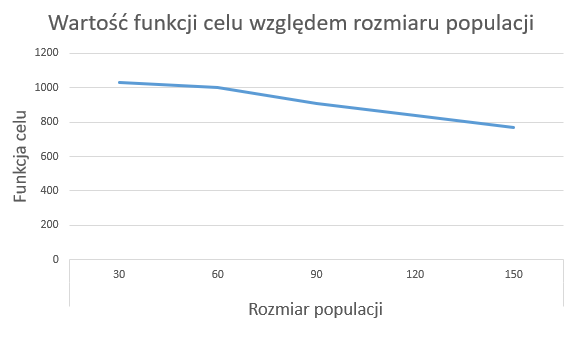
\includegraphics[scale=0.75]{Zad4_50.png}
    \centering
    \caption{Wykres zależności funkcji celu od rozmiaru populacji dla permutacji liczącej 50 miast}
  \end{figure}
  \begin{figure}[H]
    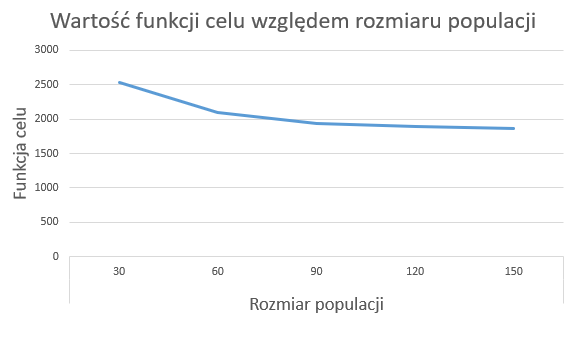
\includegraphics[scale=0.75]{Zad4_100.png}
    \centering
    \caption{Wykres zależności funkcji celu od rozmiaru populacji dla permutacji liczącej 100 miast}
  \end{figure}
  \begin{figure}[H]
    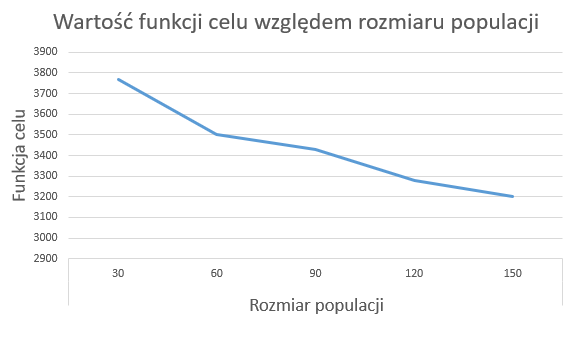
\includegraphics[scale=0.75]{Zad4_150.png}
    \centering
    \caption{Wykres zależności funkcji celu od rozmiaru populacji dla permutacji liczącej 150 miast}
  \end{figure}
  \begin{figure}[H]
    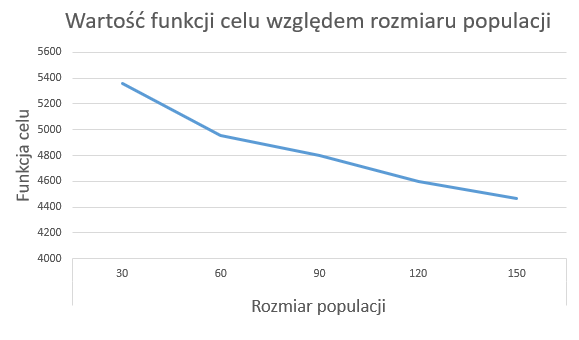
\includegraphics[scale=0.75]{Zad4_200.png}
    \centering
    \caption{Wykres zależności funkcji celu od rozmiaru populacji dla permutacji liczącej 200 miast}
  \end{figure}
  \begin{figure}[H]
    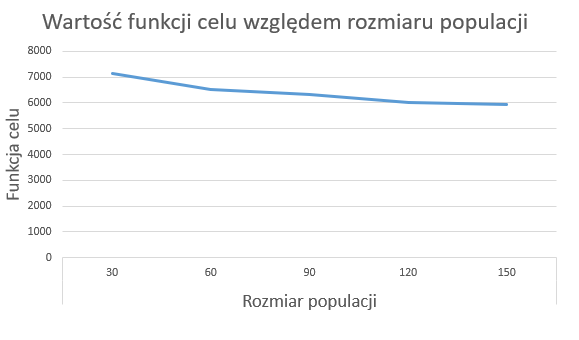
\includegraphics[scale=0.75]{Zad4_250.png}
    \centering
    \caption{Wykres zależności funkcji celu od rozmiaru populacji dla permutacji liczącej 250 miast}
  \end{figure}
  \subsection{Wnioski: }
      Zauważamy, iż zwiększenie rozmiaru populacji przy stałym utrzymaniu tych samych wariantów wpływa na uzyskanie lepszych wyników.
